%************************************************
\chapter{Introduction}\label{ch:introduction}
%************************************************
Navigation and planning are essential for mobile robots to act in out- and indoor environments. 
From self driving cars navigating 132~miles through the Mojave desert, or mobile robots handling goods in distribution centers and warehouses to mobile robots used for planetary exploration, autonomous robots have conquered nearly every place on earth and beyond.
 
Articles like \cite{stanley} and \cite{kiva} present the relationship between the environmental complexity and the computational on-board processing power needed to tackle the navigation problem.
The self driving car Stanley has a six processor computing platform provided by Intel whilst Kiva robots are using low cost DSP's for navigation and vision processing\footnote{Kiva Systems Uses "Smart" Blackfin-powered Robots for Warehouse Navigation | Analog Devices: \url{http://www.analog.com/en/content/kiva_systems_bf548/fca.html}} to drive within a known environment.  

While the application domains and computational powers varies strongly between the robotic systems, all of them have to move safely and efficient from one location to another.   

In this thesis a method for improving navigation for mobile robots by the use of combining local planning methods with search strategies based on meta-heuristics is proposed.

This enables the local planner to:
\begin{itemize}
\item run at a higher frequency
\item simulate trajectories for a longer time interval
\item moving the robot at higher speed
\item investigate a larger amount of trajectories
\item use a higher costmap resolution
\end{itemize}

In order to give an impression of the importance of navigation and planning in the field of mobile robotics the next section gives some motivation and application examples.

\section{Motivation and Applications}\label{sec:motivation} 
The goal of navigation encompasses the ability of robots to find a series of actions based on its knowledge of the environment and sensor values to reach its goal position in an effective and efficient manner.
The resulting series of actions is called a \emph{plan}. 

To ensure safety and flexibility in the presence of obstacles in a dynamic environment \emph{obstacle avoidance} is used to alter plans during execution and generating of collision free trajectories.

A common strategy to deal with complex navigation problems is to the divide the planning task into a global and a local planning problem \cite{LaValle2006}.

Global path-planning usually operates on a simplified representation of the environment and the robot itself (e.g. static map, circle representation of the robots outline) to efficiently compute an optimal shortest path using variants of Dijkstra's \cite{dijkstra1959note} or $A^*$ \cite{DBLP:journals/tssc/HartNR68/Astar} algorithm, ignoring kinematic and acceleration constraints of the robot.
In succession the retrieved global path is used by a local planner for guiding the robot through the environment.
Figure~\ref{fig:fig_pioneer} illustrates the view of the environment from a robot perspective together with a global and local plan, which enables the robot to drive autonomous within a lab/office environment.

\begin{figure}[thpb]
      \centering
      \def\svgwidth{\textwidth}
      \includesvg{figures/pioneer_costmap}
      \caption[Global and local planning.]{This figure shows a Pionner3DX and its view of the office environment while passing through a door. The blue line shows the global path and the green line the selected trajectory of the local planner.}
      \label{fig:fig_pioneer}
\end{figure}

The major responsibility for local planner is obstacle avoidance. It takes sensor readings of the robot into account and is reactive to changes within the sensor range. 
It selects the best values of available motor controls in respect to the kinematic and dynamic constraints of the robot, generating collision free trajectories. 
   
Navigation competence is essential for a broad spectrum of application domains within the field of mobile robotics which are presented below:

\begin{description}
\item[Self driving cars]\hfill \\
Self driving cars (see Figure~\ref{fig:fig_auto}) like Stanley \cite{stanley} which won the 2005 DARPA (Defense Advanced Research Projects Agency of the United States) Grand Challenge and the Google car \cite{guizzo2011google} are two examples which illustrate the enormous potential of autonomous vehicles.
While the former is confronted with rough terrain and maneuvers at high speeds, cars in urban traffic have to be prepared for other vehicles, pedestrians and have to incorporate traffic rules into the navigation task. 

\begin{figure}[thpb]
	  \myfloatalign
      \footnotesize
      \centering
    \subfloat[Stanley (taken from \cite{stanley}).]
    {  \label{fig:fig_stanley}
        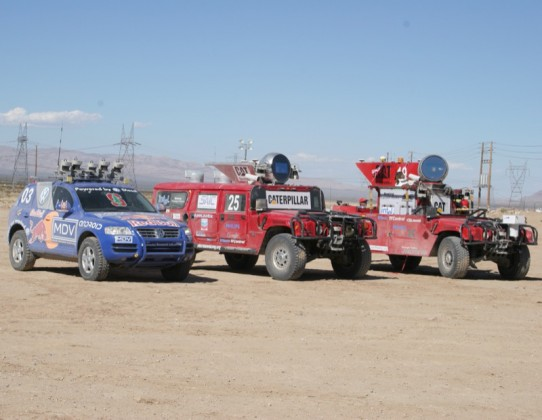
\includegraphics[width=0.45\textwidth,height=0.2\textheight]{figures/fig_stanley.jpg}
    }    
    \subfloat[Google car (Credit: Google\protect\footnotemark).]
    {  \label{fig:fig_googlecar}
       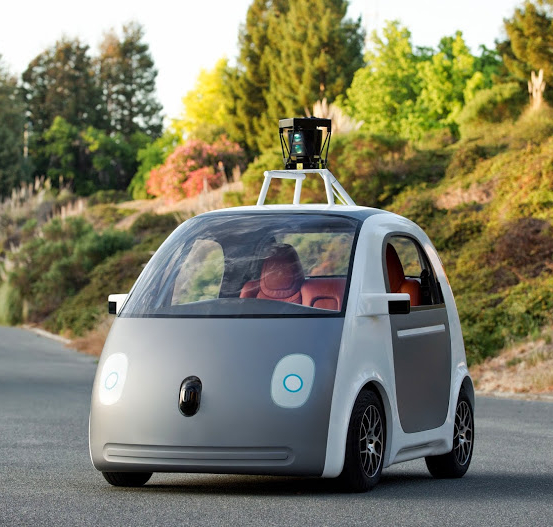
\includegraphics[width=0.35\textwidth,height=0.2\textheight]{figures/fig_googlecar.jpg}
    }
   \caption[Selfdriving car]{Self driving cars designed for different environments. On the left the winner of the 2005 DARPA Grand Challenge tackled wreckless driving through the Mojave desert and the right picture shows the new Google car designed for urban traffic.}
   \label{fig:fig_auto}
\end{figure}

\item[Planetary exploration]\hfill \\
Another example of autonomous vehicles are planetary rovers.
Three generations of Mars rovers developed at NASA are shown in Figure~\ref{fig:fig_nasa}. 
The first Mars rover, Sojourner, which landed on Mars in 1997 as part of the Mars Pathfinder Project was remotely operated from earth. 
The next generation of rovers, Spirit and Opportunity which landed 2004, did already have an autonomous navigation system. This enabled the robots to avoid hazardous situations without human intervention. 
The latest rover Curiosity is on its mission on Mars since August 2012 using autonomous navigation to explore mars on safe paths without the need of being remotely controlled by human operators.

An overview of recent developments in the field of planetary exploration including navigation topics can be found in \cite{PavoneAcikmese2014rover}.

\begin{figure}[thpb]
	  \myfloatalign
      \footnotesize
      \centering
    \subfloat[NASA Mars rover (Credit: NASA JPL-Caltech).]
    {  \label{fig:fig_nasa}
        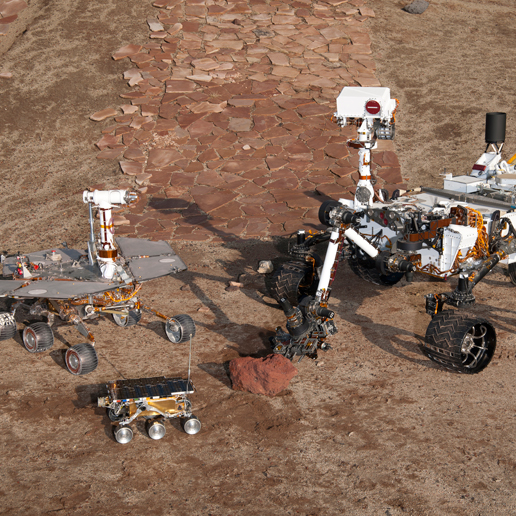
\includegraphics[width=0.35\textwidth,height=0.2\textheight]{figures/fig_marsrover.jpg}
        %\caption{Dijkstra}
    }
    \subfloat[Mawson rover (taken from \cite{Allister2012rover}).]
    {  \label{fig:fig_rover}
        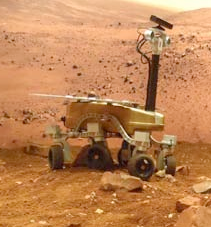
\includegraphics[width=0.35\textwidth,height=0.2\textheight]{figures/fig_rover.png}
        %\caption{Dijkstra}
    }     
   \caption[Mars rover]{Different Mars rover for planetary exploration. On the left Sojourner, Spirit and Curiosity from NASA which provided rich scientific information exploring Mars and on the right Mawson an academic research project on a training track at the Museum of Sydney.}
   \label{fig:fig_rovers}
\end{figure}
\footnotetext{Google self driving car available from \url{http://googleblog.blogspot.co.at/2014/05/just-press-go-designing-self-driving.html}}

\item[Search and Rescue]\hfill \\
Mobile robots provide a useful tool for rescue teams, whenever human intervention is not possible due to imminent risk of health and life, like immediate explosion hazard or threat of nuclear radiation.  
Figure~\ref{fig:fig_rescue} shows two prominent representatives of search and rescue robots.
\begin{figure}[thpb]
	  \myfloatalign
      \footnotesize
      \centering
    \subfloat[Pioneer (Credit: Carnegie Mellon University)]
    {  \label{fig:fig_chernobyl}
        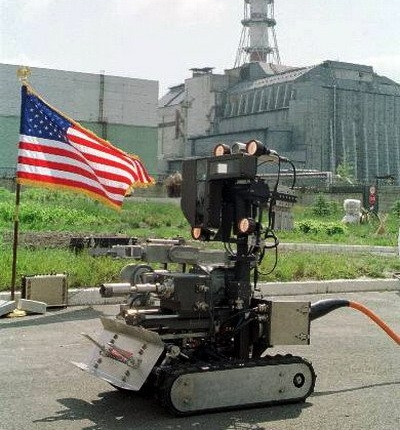
\includegraphics[width=0.35\textwidth,height=0.2\textheight]{figures/fig_chernobyl_pioneer.jpg}
        %\caption{Dijkstra}
    }
    \subfloat[Packbot (Credit: iRobot)]
    {  \label{fig:fig_fukushima}
        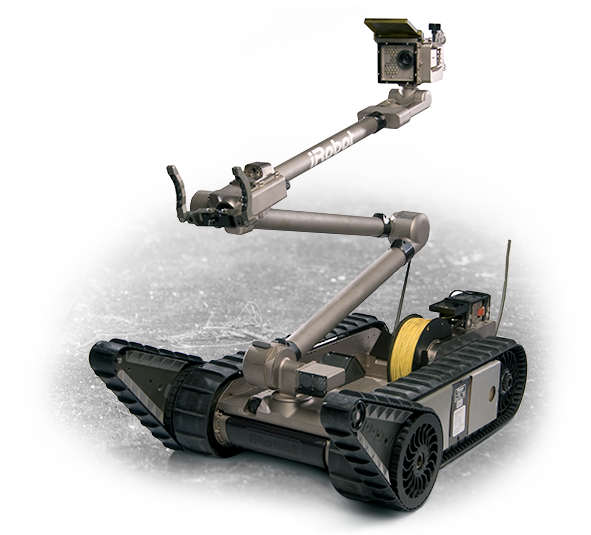
\includegraphics[width=0.35\textwidth,height=0.2\textheight]{figures/fig_packbot.png}
        %\caption{Dijkstra}
    }     
   \caption[Rescue robots]{Search and rescue robots are useful tools for human rescue teams. The left figure shows Pioneer at the nuclear disaster site in Chernobyl, the right robot shows a Packbot which operated in the nuclear power plant in Fukushima.}
   \label{fig:fig_rescue}
\end{figure}

The robot PIONEER sponsored by the US Department of Energy and NASA was the first of its kind to be deployed to the remnants of the nuclear power station in Chernobyl in the Ukraine after the supergau in 1986. 
The robots mission was to evaluate the sarcophagus which was built to shield off radiation.

In 2011 after an earthquake caused a nuclear disaster at the Fukushima Daiichi power plant in Japan, two PACKBOT robots of the American company iRobot were deployed to perform on site observations.

While the aforementioned robots were remotely operated, autonomous robots are a hot research topic in the academic domain. In the last 5 years more than 90 teams from universities participated in RoboCup competitions and already provide impressive results like Hector \cite{2014:hector_rescue_tdp} the winner of the 2014 RoboCup Rescue League world championship.

\item[Assistance]\hfill \\
Besides robots acting in outdoor environments, assistance robots have to cope with the difficulties involved in operating side by side with humans in indoor environments. 
Obstacles like desks and chairs located in small corridors and rooms pose a challenging navigation problem.
Tour guide robots like Rhino \cite{DWA1997} and Robox \cite{philippsen:2004:phd} are especially designed to deal with this kind of setting.
Figure~\ref{fig:fig_robox} shows Robox at the Robotics@Expo.02 event. 

Figure~\ref{fig:fig_hobbit} shows the robot Hobbit \cite{fischinger2013hobbit}\cite{zagler2014roboter} which goes one step further in assisting elderly people in their everyday activities.
It does not only make an excellent job in dealing with the pitfalls of navigating in indoor environments, in addition it is equipped with the capabilities to identify and to remove obstacles on the floor to provide safe passages for its human users.

\begin{figure}[thpb]
	  \myfloatalign
      \footnotesize
      \centering
    \subfloat[Hobbit (taken from \cite{fischinger2013hobbit})]
    {  \label{fig:fig_hobbit}
        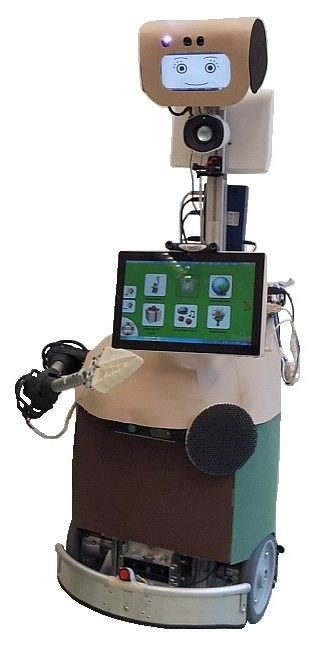
\includegraphics[width=0.30\textwidth,height=0.34\textheight]{figures/fig_hobbit.png}
        %\caption{Dijkstra}
    }
    \subfloat[Robox (taken from \cite{philippsen:2004:phd})]
    {  \label{fig:fig_robox}
        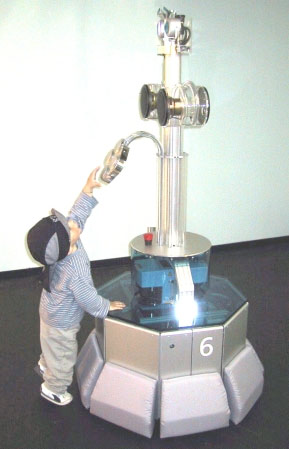
\includegraphics[width=0.30\textwidth,height=0.34\textheight]{figures/fig_robox.png}
        %\caption{Dijkstra}
    }     
   \caption[Assitance robots]{Hobbit the \emph{care} robot supporting elderly people and Robox working as a tour guide.}
   \label{fig:fig_assist}
\end{figure}

\item[Logistics and Transportation]\hfill \\
Automated guided vehicles (AGV) are an essential part in industry to support automated manufacturing. Figure~\ref{fig:fig_agv} shows a typical industrial AGV from the Austrian company DS-Automotion.
The mobile robots follow markers, wires, or magnets in the floor, and make use of lasers and computer vision methods to accomplish navigation tasks. 
Their main responsibility is to move materials safely and efficient around manufacturing facilities, warehouses (eg. Kiva Systems \cite{kiva}) or hospitals (eg. HELPMATE \cite{ROB:4520696}). 

If transportation by road is not possible a flying drone might do the job. Projects from major companies like Googles \emph{project wing}\footnotetext{Project Wing delivery drones \url{https://plus.google.com/+google/posts/TqrsvRyPeNH}} and Amazons \emph{Prime Air} are working on self flying drones to deliver packages. 
Figure~\ref{fig:fig_uav} shows a prototype drone on a test flight. 

\begin{figure}[thpb]
	  \myfloatalign
      \footnotesize
      \centering
    \subfloat[AGV (Credit: DS-Automotion)]
    {  \label{fig:fig_agv}
        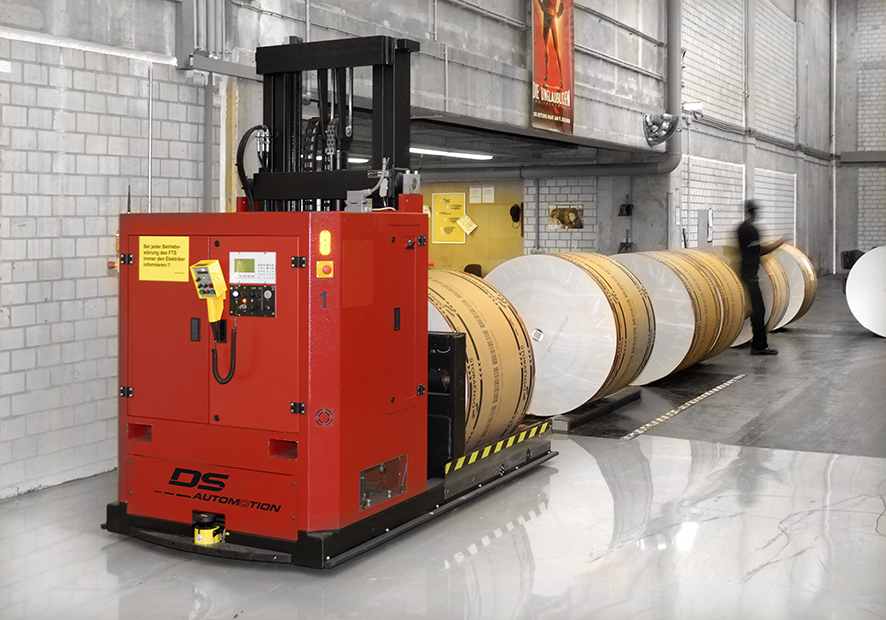
\includegraphics[width=0.35\textwidth,height=0.2\textheight]{figures/fig_AGV-dsautomation.jpg}
        %\caption{Dijkstra}
    }
    \subfloat[Project Wing delivery drone (Credit: KEYSTONE)]
    {  \label{fig:fig_uav}
        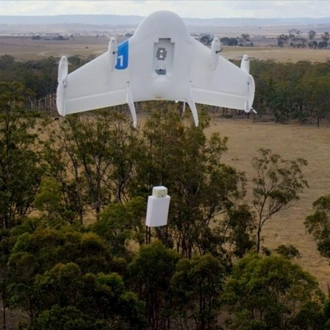
\includegraphics[width=0.35\textwidth,height=0.2\textheight]{figures/fig_wing.jpg}
        %\caption{Dijkstra}
    }     
   \caption[Logistic robots]{Transportation on earth using Automated Guided Vehicles and in the air with the support of self flying drones.}
   \label{fig:fig_transport}
\end{figure}

\item[Commercial]\hfill \\
Robots play a vital role in the manufacturing of goods. Besides classical domains such as  automotive industry, robots are used for mining, construction and maintenance tasks. 
For example DeWaLoP, shown in figure~\ref{fig:inpipe}, is used for cleaning fresh water pipes, navigating through a 3000 km pipeline network in Vienna \cite{mateos2013inpipe}.   

The employment of autonomous robots is also a field of attention in agriculture. 
Monitoring, harvesting and precision spraying pesticides of crops have to be carefully accomplished without hurting fragile plants. 
Figure \ref{fig:fig_cropbot} shows a harvesting robot developed at the Technische Universit\"at M\"unchen moving in a greenhouse \cite{Schuetz2014}.

\begin{figure}[thpb]
	  \myfloatalign
      \footnotesize
      \centering
    \subfloat[DeWaLoP (taken from \cite{mateos2013inpipe})]
    {  \label{fig:inpipe}
        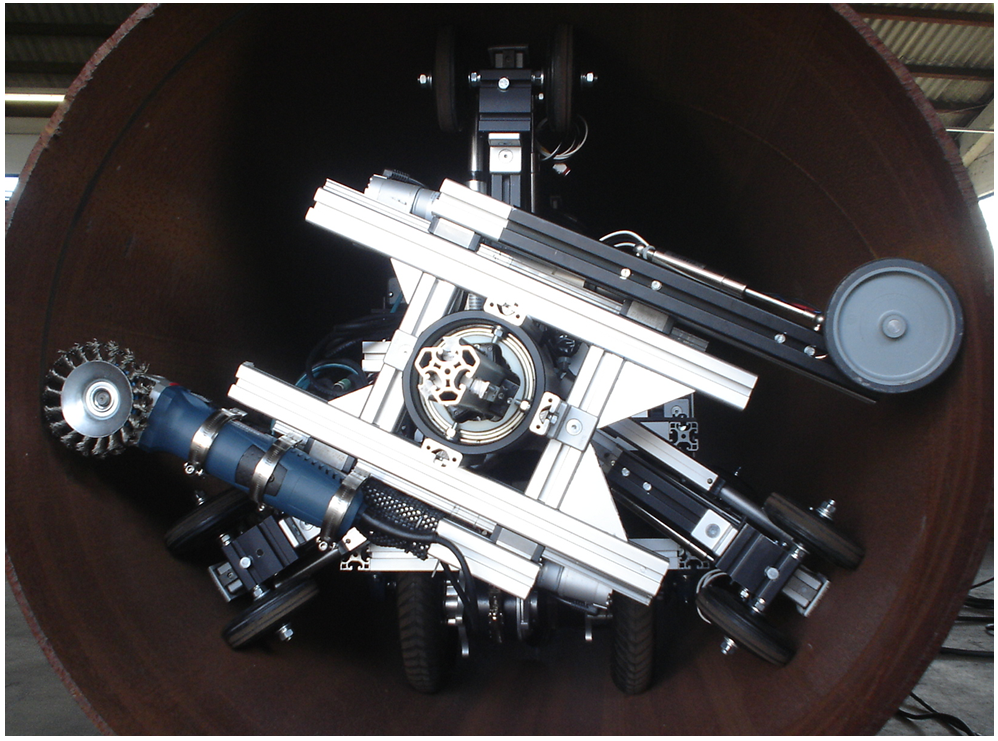
\includegraphics[width=0.35\textwidth,height=0.2\textheight]{figures/fig_inpiperobot.png}
        %\caption{Dijkstra}
    }
    \subfloat[Harvesting robot (taken from \cite{Schuetz2014})]
    {  \label{fig:fig_cropbot}
        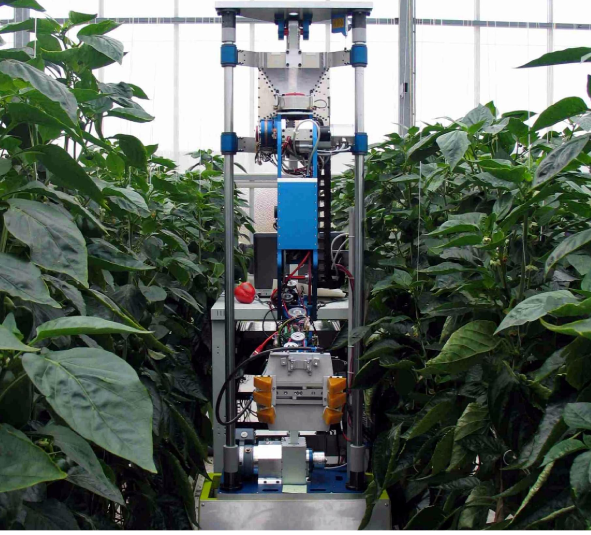
\includegraphics[width=0.35\textwidth,height=0.2\textheight]{figures/fig_croprobot.png}
        %\caption{Dijkstra}
    }     
   \caption[Commercial robots]{The right figure shows an in-pipe maintenance robot, the left image an agricultural robot used for harvesting and spraying of sweet-pepper crops.}
   \label{fig:fig_commercial}
\end{figure}

\item[Challenges and Competitions]\hfill \\
Attractive competitions have the purpose to spur innovation and sponsor research development in the field of robotics .  
One of the most popular events are organized and sponsored by DARPA. Besides the already mentioned Grand Challenge for wreckless self driving cars, the successor events DARPA Urban Challenge focused on autonomous vehicles moving in urban areas. 
In 2012 the first DARPA Robotics Challenge took place which provided a platform for wheeled and humanoid search and rescue robots.

World Competitions of soccer playing robots fascinate and motivate thousands of people every year and have a significant impact on the development of innovative methods including navigation and planning for mobile robots.
Figure~\ref{fig:fig_competition} shows wheeled and humanoid robots trying their best at scoring more goals than their opponents.
The biggest events are organized by FIRA\footnote{Federation of International Robot-soccer Association, founded in 1997. Details can be found at \url{www.fira.net}.} and RoboCup\footnote{RoboCup Federation, founded in 1993. Details can be found at \url{www.robocup.org}.}, which provide annual competitions for wheeled and humanoid soccer robots.

\begin{figure}[thpb]
	  \myfloatalign
      \footnotesize
      \centering
    \subfloat[MiroSot (taken from \url{www.fira.net})]
    {  \label{fig:mirosot}
        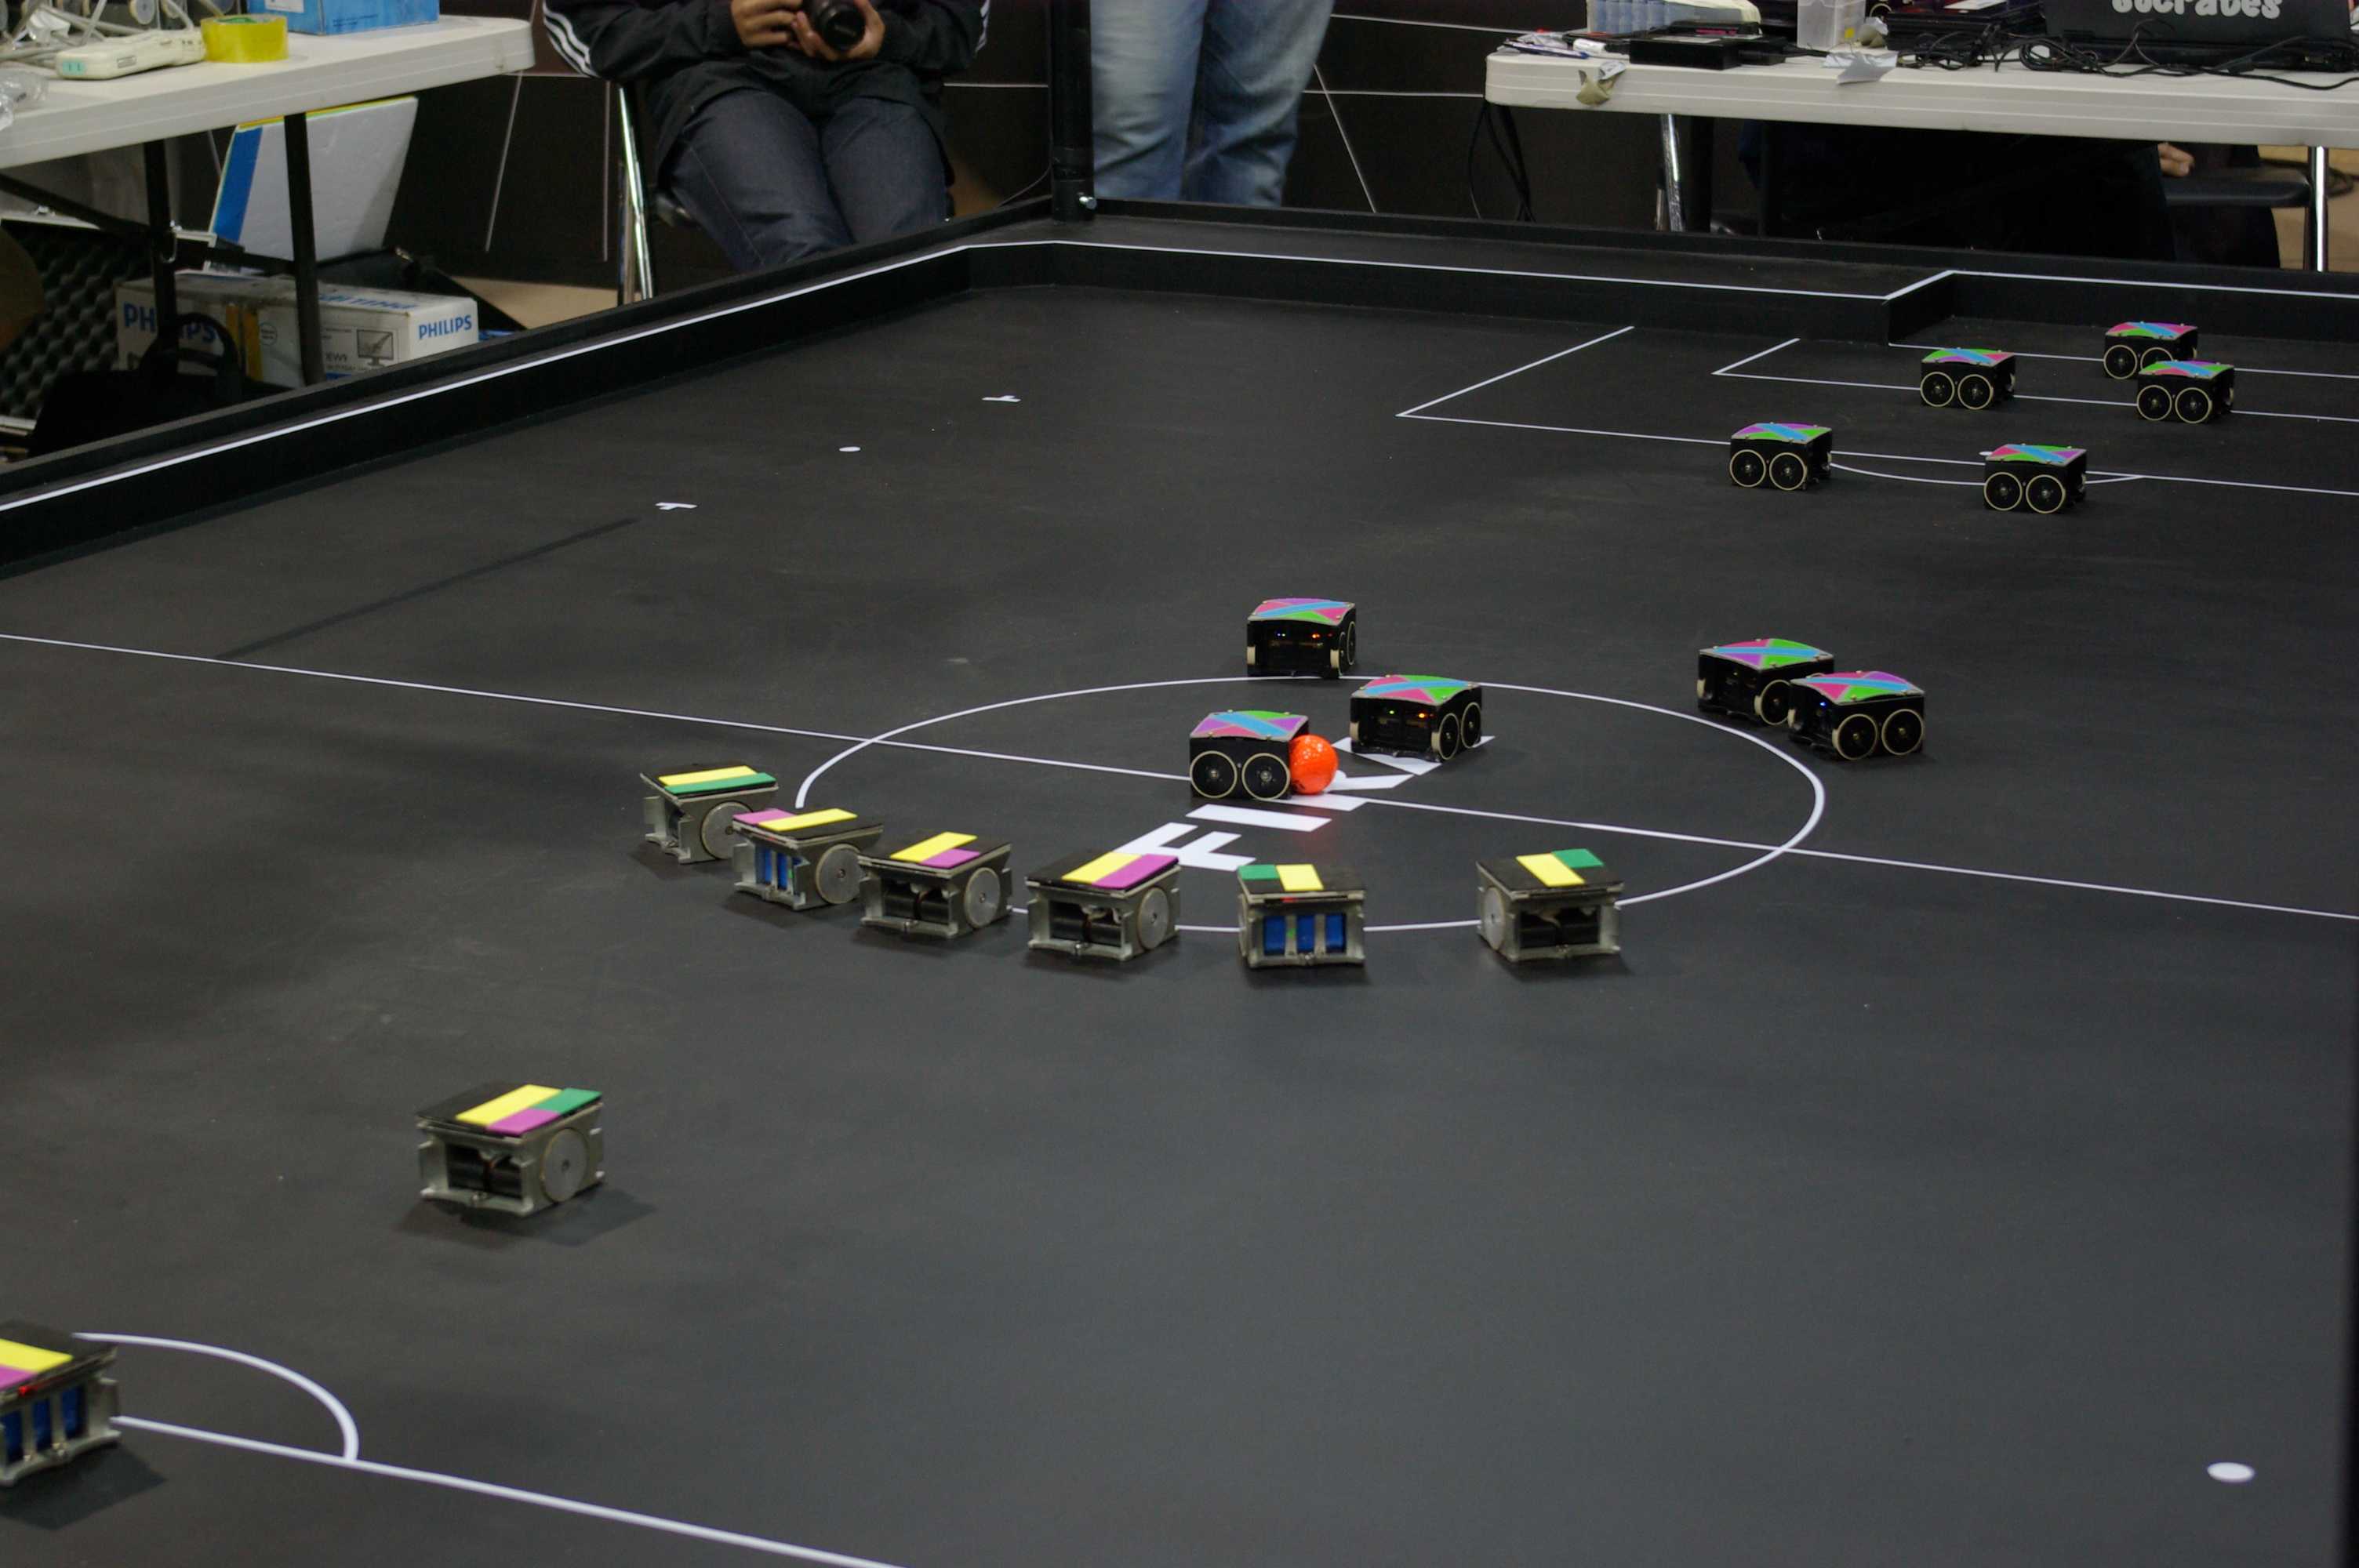
\includegraphics[width=0.35\textwidth,height=0.2\textheight]{figures/fig_mirosot.jpg}
        %\caption{Dijkstra}
    }
    \subfloat[Standard Platform League (taken from \url{www.robocup2014.org})]
    {  \label{fig:fig_naosoccer}
        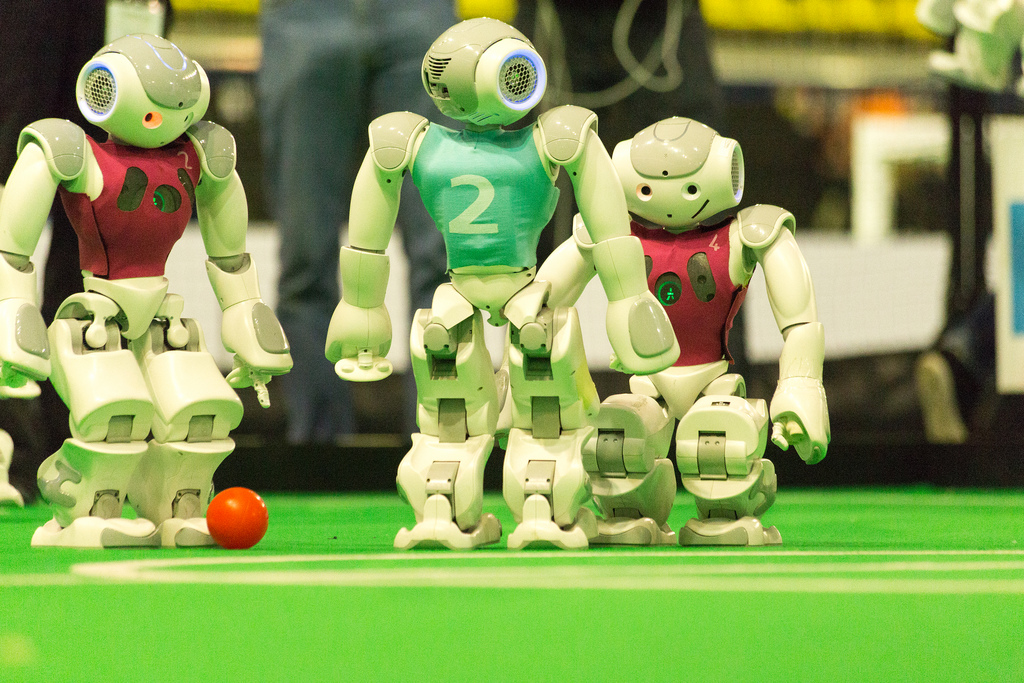
\includegraphics[width=0.35\textwidth,height=0.2\textheight]{figures/fig_naosoccer.jpg}
        %\caption{Dijkstra}
    }     
   \caption[Soccer robots]{The right figure shows competitors of the MiroSot league, the left image humanoid Nao robots playing soccer in the RoboCup Standard Platform League.}
   \label{fig:fig_competition}
\end{figure}
\end{description}

All of these examples show that navigation plays an essential role in mobile robotics. Excellent planning algorithms are needed to enable a wide area of applications and allow autonomous and semi-autonomous machines to safely and economically move through in- and outdoor environments.
In addition they have to cope with uncertainties induced by sensor noise, the presents of dynamic obstacles and the limits of computational power.

\section{Related Work}\label{sec:relwork}
Similar approaches using meta-heuristics are mostly present in the field of global planning. Especially population based meta-heuristic algorithms are used to tackle planning problems for single and multiple robots.

In \cite{zhou2010improvedantcolony} an ant colony optimization (ACO) algorithm is used to find global minimal paths for soccer robots. 
The algorithm uses a combination of cellular automata and a special designed pheromone model to find an initial global path. 
In a second step the retrieved path is smoothed and can be used to guide a robot.

In \cite{buniyamin2011robotantcolony} the performance of finding optimal shortest global paths by applying an ACO algorithm is documented. 
The proposed method uses a special heuristic to set the moving directions of the ants in the system based on shortest distance between nodes in the search graph.  

A combination of a local planner based on artificial potential field method and a global planner based on ACO is presented in \cite{mei2006hybrid}. 
Here the pherhormon traces of the ACO is used to prevent local minima in the local planning step.

Several approaches using genetic programming are presented in \cite{manikas2007genetic} where solutions to planning problems for autonomous navigation are encoded as chromosomes. 
According to a fitness function the best chromosomes are chosen to create new solutions via cross over and mutation operations. 

An early apporach of using single solution based meta-heuristics in the context of local planning is presented in \cite{park2001obstacle}.
Here simulated annealing was applied to avoid the local planner of getting trapped in local minima.

Based on tabu search a sensor based navigation system for mobile robots is presented in \cite{masehian2008sensor}.
This local planning method utilizes different memory structures to avoid cycling back to already visited regions of the map. 
To escape local minima it provides an escaping mechanism by randomly approaching unvisited areas.

The method proposed in this work differs from these works by analyzing and using single solution based meta-heuristics strategies for local path planning only. 
In addition to the memory structures of tabu search, another contribution is the use of algorithms based on Iterated Local Search (ILS) and Variable Neighborhood Search (VNS). 
These single solution based meta-heuristics are the core strategies to increase the efficiency of a local planner which uses trajectory generation methods like the Dynamic Window Approach (DWA) to find optimal motor controls for the robot.

\section{Goal of Thesis and Scientific Contribution}\label{sec:goal}
The goal of this thesis is to provide an extension to local planning systems for mobile robots based on trajectory generation and parts of this work were presented at the Austrian Robotics Workshop 2014 \cite{myself}. 
The proposed method applies meta-heuristic search strategies to improve the performance of local planner based on brute force evaluation of a fixed number of trajectories.

This includes the following sub-goals.
\begin{description}
\item[Compilation of local planning approaches]\hfill \\
A detailed overview of local planning and obstacle avoidance methods has to be compiled. 
\item[Investigating possible meta heuristic algorithms]\hfill \\
Selection and adapting applicable meta-heuristics to make them usable for trajectory selection.
\item[Design of benchmark instances and sample planner]\hfill \\
Suitable test instances and a sample planning program which allow to set the focus of investigating the proposed method on the local planning task have to be developed.  
\item[Implementation]\hfill \\
The gained data from the benchmark instances and the sample planner are used to implement meta-heuristic local planning in an existing navigation system for mobile robots.  
\item[Evaluation]\hfill \\
Experiments have to be designed and evaluated to document the performance of the meta-heuristic algorithms in comparison to their unaltered counterparts.
\end{description}

\section{Outline}\label{sec:outline}
This work is structured in the following way. 
%In Chapter \ref{ch:introductionplanning} the basic sources for planning are outlined, covering the basic problem definition, representation of the environment and different robotic motion models. 
Chapter \ref{ch:local} gives an overview of important local planning and obstacle avoidance methods.
 
Chapter \ref{ch:meta} represents the main part of this thesis and introduces meta-heuristic extensions to local planning methods. 
Starting with an detailed overview of  meta-heuristic algorithms, two application based on ILS and VNS are used for trajectory selection of a local planner and described in Section \ref{sec:trajselmeta}.

A detailed evaluation of these methods is presented in Chapter \ref{ch:eval}, using a very simple implementation of a local planner and randomly generated sensor maps. 
The gathered data is then used to implement a meta-heuristic trajectory selection in a high sophisticated planner and tested using simulation software with a robust physical engine.

Chapter \ref{ch:conc} concludes the work of this thesis with a short summary and an outlook on future research directions.
%*****************************************
%*****************************************
%*****************************************
%*****************************************
%*****************************************




